\documentclass[12pt,a4paper]{article}

\usepackage{german}      % Deutsche TeX-Eigenheiten
%\usepackage{isolatin1}   % Eingabekodierung mit Umlauten...

\usepackage{makeidx}
\makeindex            % damit eine Indexdatei angelegt wird

\usepackage{graphicx}

\usepackage{amsmath}  % allgemeine Mathe-Erweiterungen
\usepackage{amssymb}  % Symbole und Schriftarten
\usepackage{amsthm}   % erweiterte Theorem-Umgebungen

\usepackage{mathrsfs}  % gibt den Befehl "\mathscr{}" für schöne

\usepackage[noframe]{showframe}
\usepackage{framed}
\renewenvironment{shaded}{%
	\def\FrameCommand{\fboxsep=\FrameSep \colorbox{shadecolor}}%
	\MakeFramed{\advance\hsize-\width \FrameRestore\FrameRestore}}%
{\endMakeFramed}
\definecolor{shadecolor}{gray}{0.75}

\newcommand\underrel[2]{\mathrel{\mathop{#2}\limits_{#1}}}

\begin{document}
\section{L'Hospital}
\textbf{1. Regel} Bei \textcolor{red}{$\frac{0}{0}$}:$\lim\limits_{x\rightarrow x_0}\frac{f(x)}{g(x)}=\lim\limits_{x\rightarrow x_0}\frac{f'(x)}{g'(x)}$\\
\textbf{2. Regel} Bei \textcolor{red}{$\frac{a}{\infty}$}:$\lim\limits_{x\rightarrow x_0}\frac{f(x)}{g(x)}=\lim\limits_{x\rightarrow x_0}\frac{f'(x)}{g'(x)}$\\
Umformen bei: $0\cdot\infty, 0^0,\infty,1^\infty,\infty-\infty$\\
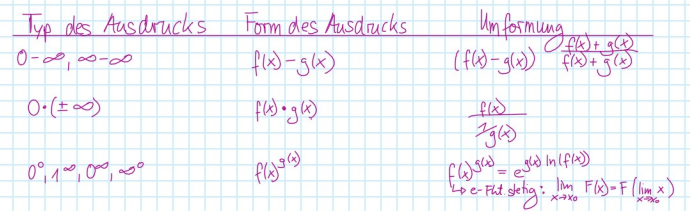
\includegraphics[width=0.8\textwidth]{Bilder/Zusfa/1.png}
\section{Taylor}
Formel:
$$
\begin{matrix}
f(x)=\underbrace{f(x_0)+\frac{f'(x_0)}{1!}\left(x-x_0\right)+\frac{f''(x_0)}{2!}\left(x-x_0\right)^2...+\frac{f^{(n)}(x_0)}{n!}\left(x-x_0\right)^n}_{\text{Taylorpolynom n-ter Ordnung (Hauptteil)}}\\
\\
+\underbrace{\frac{f^{(n+1)}(\xi)}{\left(n+1\right)!}\left(x-x_0\right)^{n+1}}_{R_n \text{Restglied von Lagrange}}
\end{matrix}
$$

Entwicklungspunkt $x_0$ = beliebig, aber fest aus Intervall\\
Zwischenstelle $\xi$ liegt zwischen x und $x_0$, kann also kleiner als x oder auch größer sein.\\
\subsubsection{Fehlerabschätzung}
worst case: $\xi$ zwischen $x_0$ und $x$ so wählen, dass $|R_n(x)|$ größtmöglich wird.\\
$$
\begin{matrix}
\Rightarrow\left|f(x)-P_n(x)\right|=\left|R_n(x)\right| &=& \left|\frac{1}{\left(n+1\right)!}f^{(n+1)}(\xi)\left(x-x_0\right)^{n+1}\right| \\
\\
&=& \frac{1}{\left(n+1\right)!}\left|\left(x-x_09\right)^{n+1}\right|\left|f^{(n+1)}(\xi)\right| \\
\\
&\leq& \frac{1}{\left(n+1\right)!}\left|\left(x-x_09\right)^{n+1}\right| M \\
\end{matrix}
$$
\newpage
Man sieht:\\
1. Je größer das n, dest kleiner wird der Faktor $1\frac{1}{(1-n)!}$\\
auf Deutsch: mit Großerem n wird die approximation besser\\
2. Je weiter das x von $x_0$ weg liegt, desto größer wird der Bertrag $x-x_0$, \\
desto mehr Einfluss hat der Term auf die Genauigkeit\\
\end{document} 